\section{Pestaña para importar del DOG}
\label{PBusquedaDOG}

\begin{figure}[H]
\centerline{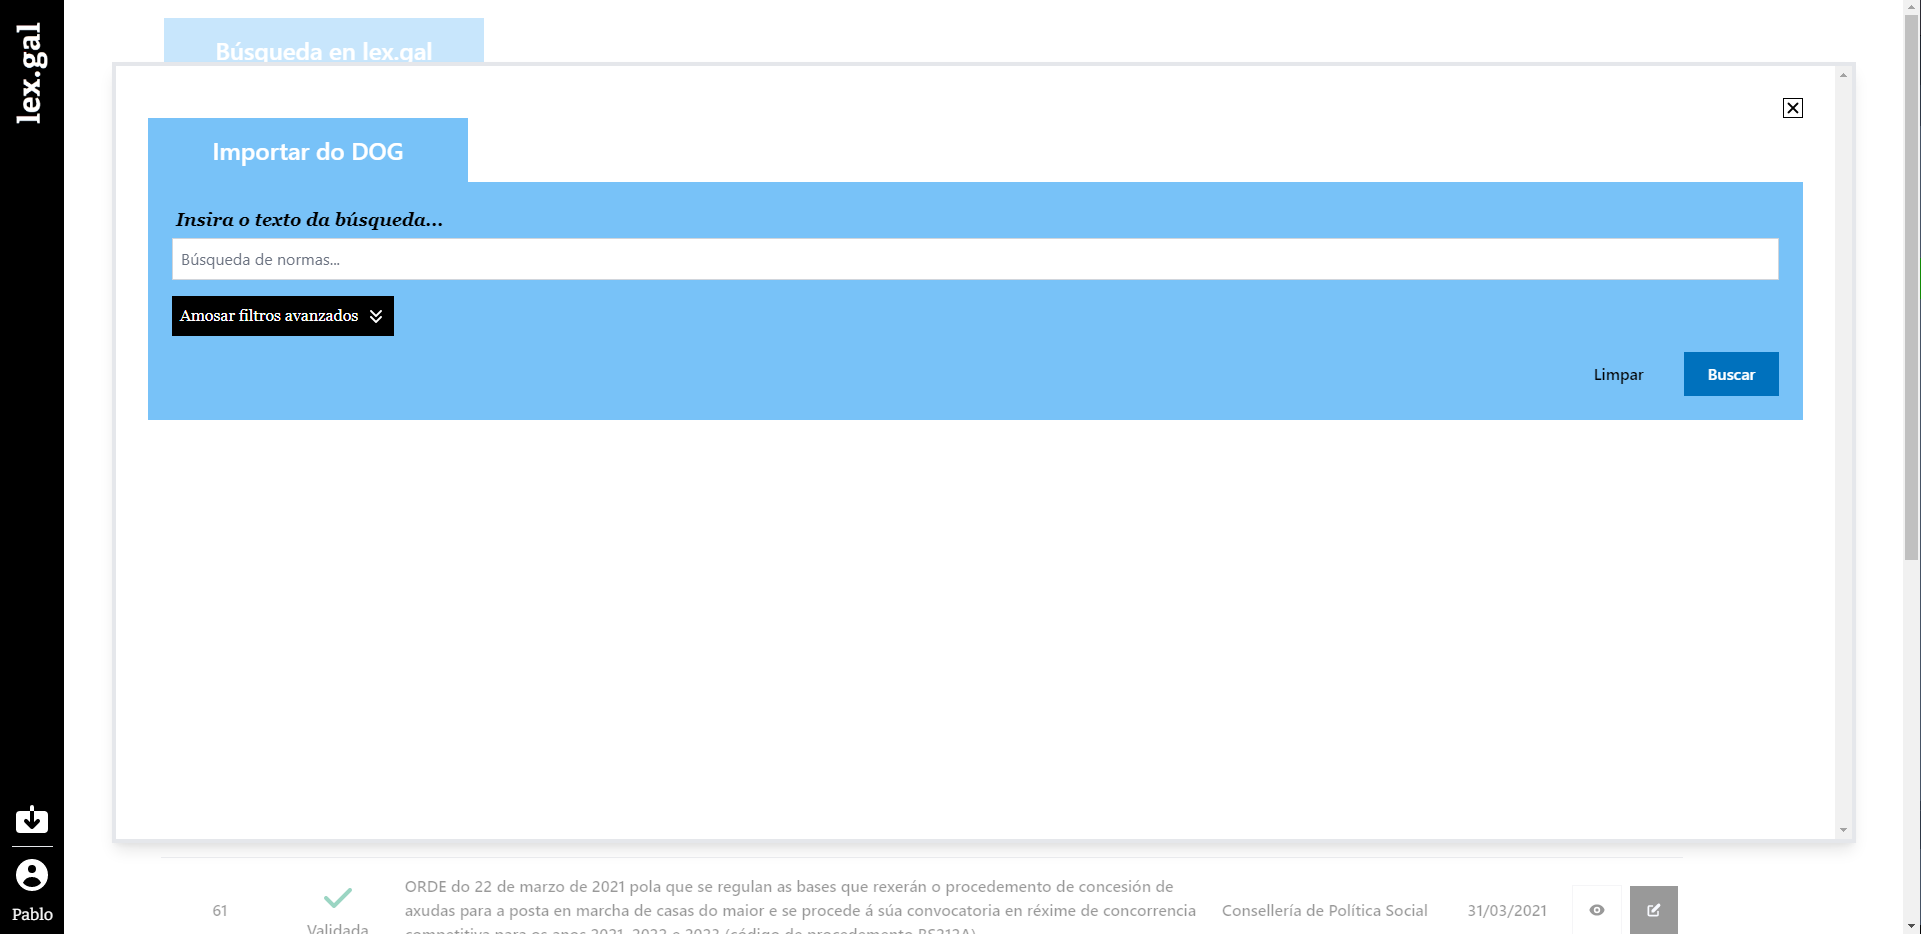
\includegraphics[width=12cm]{figuras/manualUsuario/BuscarDOG.PNG}}
\caption{Pestaña para importar del DOG - I.}
\label{enlacePBusquedaDOG}
\end{figure}

En esta pestaña, \hyperref[enlacePBusquedaDOG]{Figura B.5}, se permite buscar leyes en el DOG. Al igual que en la búsqueda de la página principal, tenemos un campo de texto, un botón para limpiar el campo, y el propio botón de buscar. Si pinchamos en ``Amosar filtros avanzados'', se mostrarán una serie de filtros a la hora de realizar la búsqueda en el DOG.
\\

Una vez realizada la búsqueda, se deberá ver algo semejante a lo siguiente:

\begin{figure}[H]
\centerline{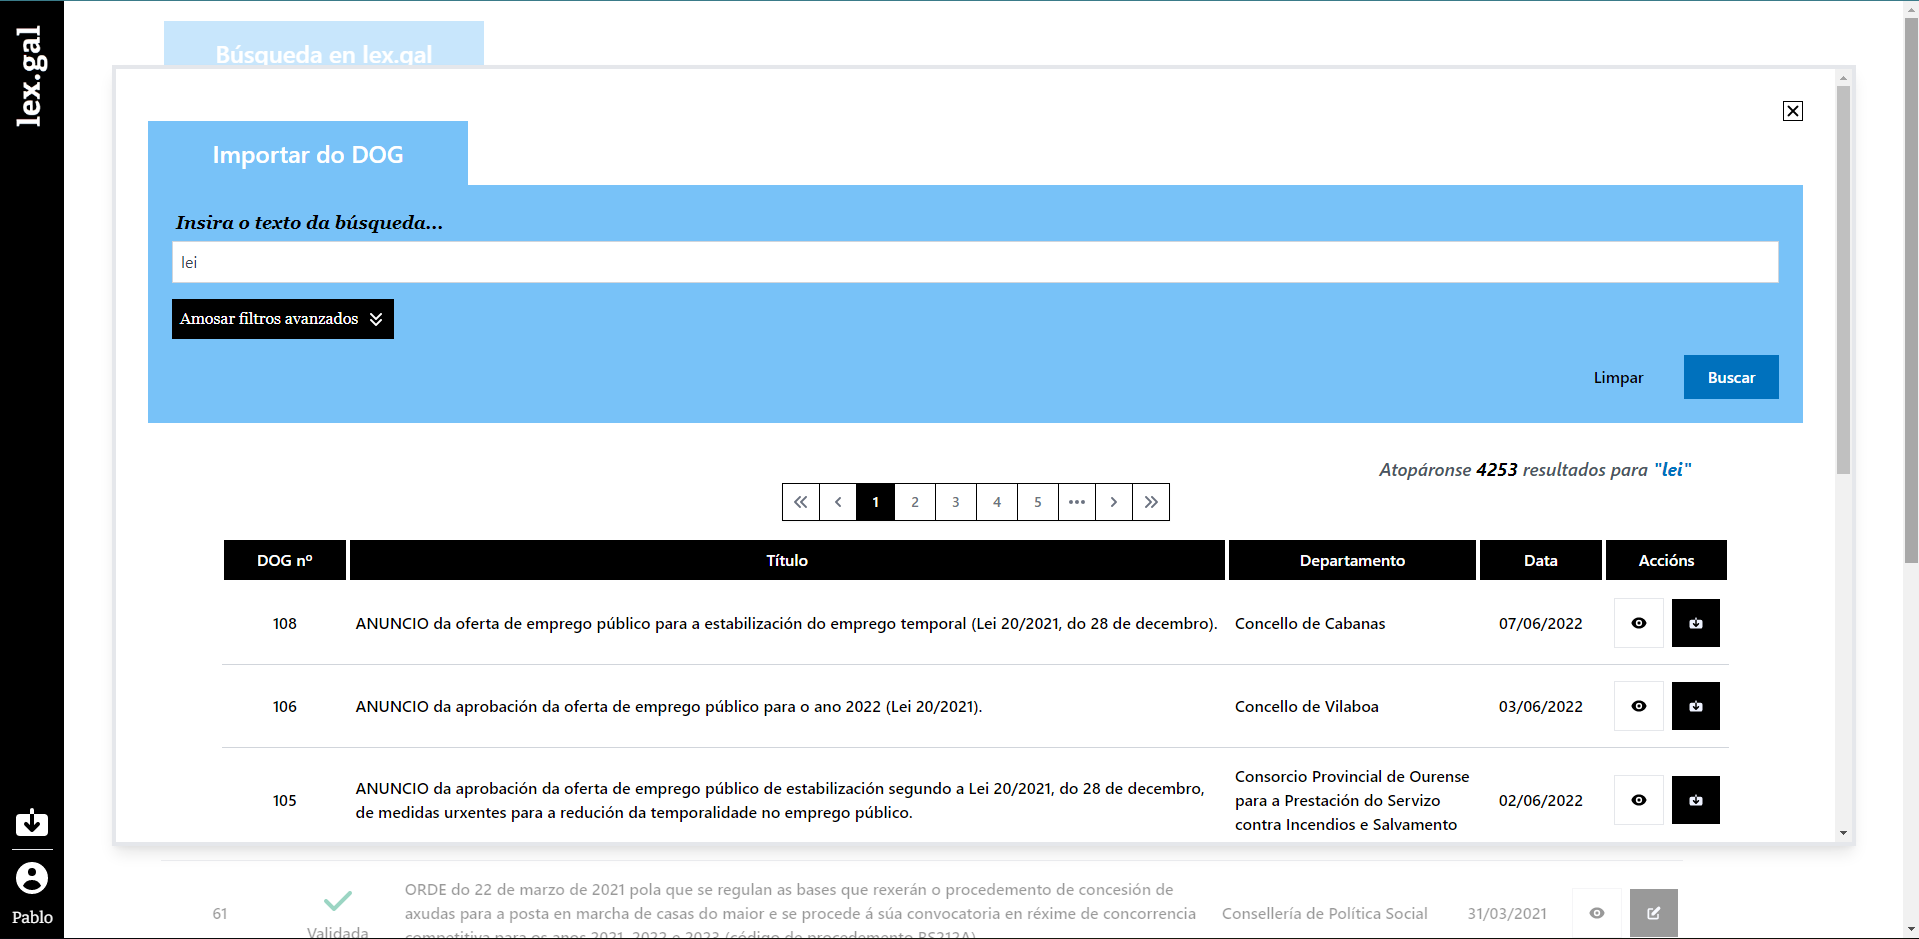
\includegraphics[width=12cm]{figuras/manualUsuario/BuscarDOGCompleta.PNG}}
\caption{Pestaña para importar del DOG - II.}
\label{enlacePBusquedaCDOG}
\end{figure}

En la \hyperref[enlacePBusquedaCDOG]{Figura B.6} se muestra una tabla con las leyes del DOG encontradas, donde encontramos una serie de acciones por cada ley. Si se pincha en el botón del ojo, se podrá previsualizar la ley en el propio DOG, como se puede observar:

\begin{figure}[H]
\centerline{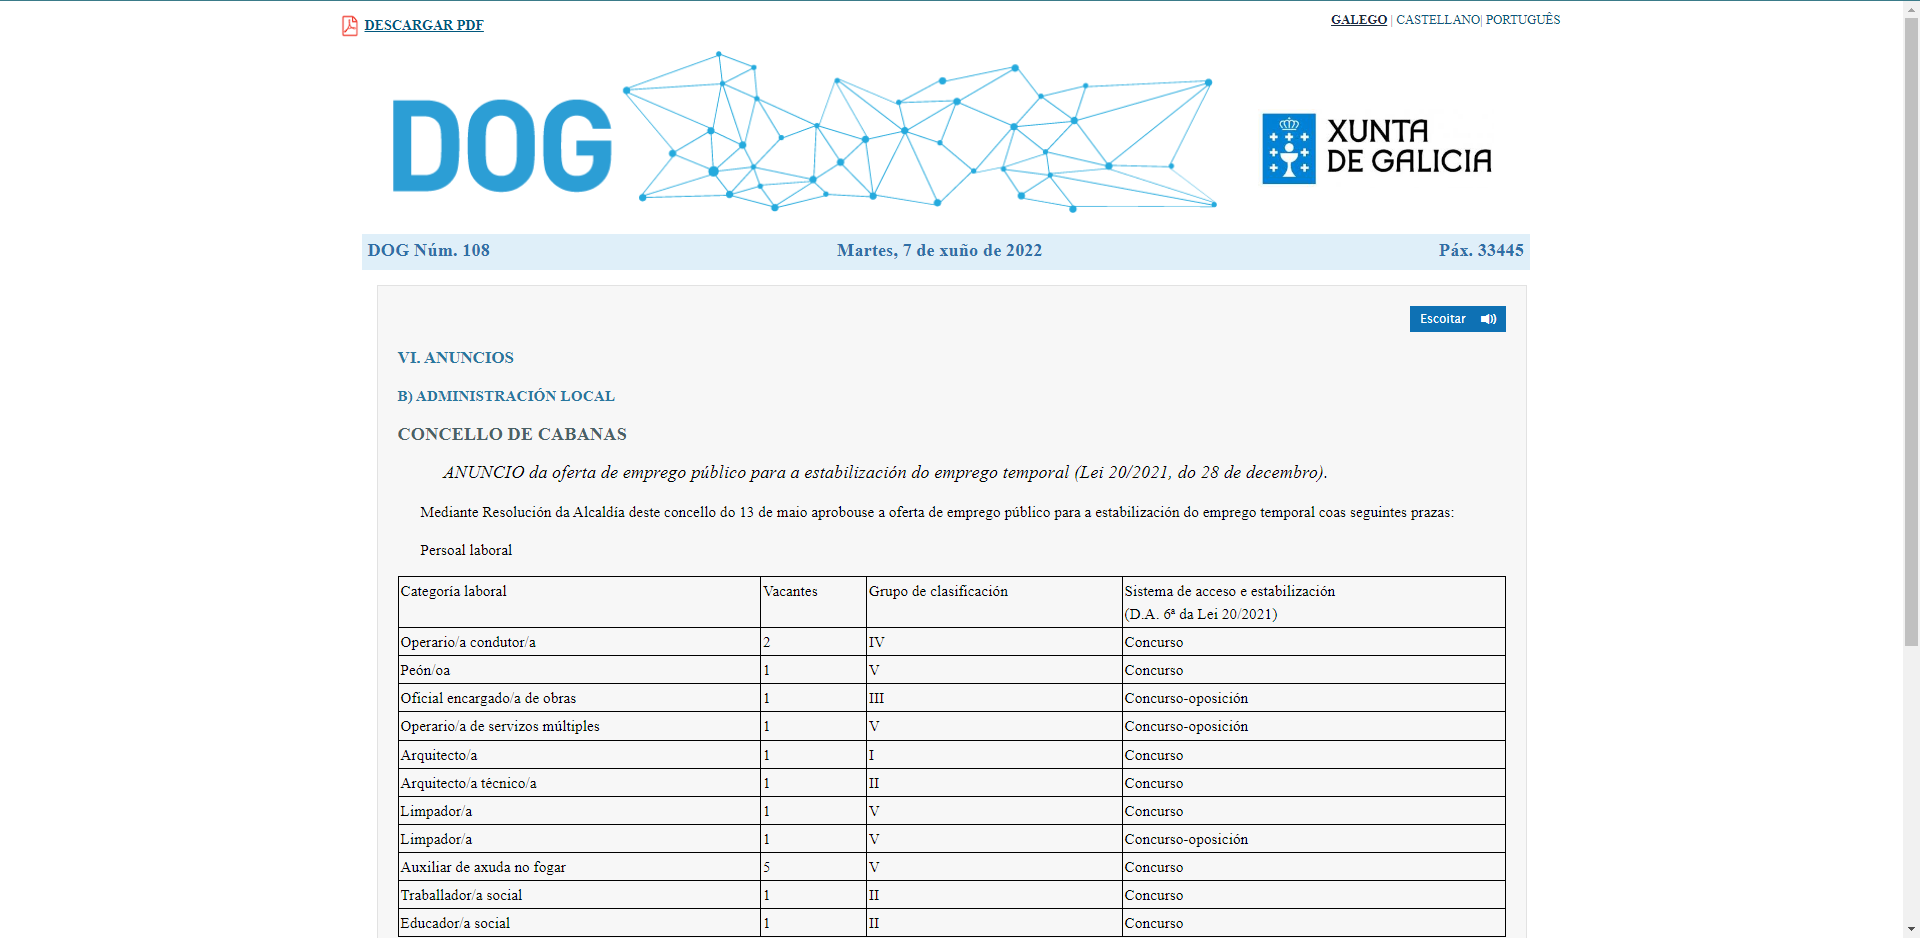
\includegraphics[width=12cm]{figuras/manualUsuario/PrevisualizarDOG.PNG}}
\caption{Previsualización de ley del DOG.}
\label{enlacePrevisDOG}
\end{figure}

En el caso de pinchar en el botón con una flecha hacia abajo de la \hyperref[enlacePrevisDOG]{Figura B.7}, se importará una ley a la aplicación de lex.gal, pasando a estar disponible en la página principal del programa.